\section{Continuous Integration overview}

\begin{frame}{Continuous Integration of Scientific Software}
    \framesubtitle{Research Software Workflow I} 
    \vfill

    \begin{columns}
        \begin{column}[c]{0.5\textwidth}
            \begin{figure}
                \centering
                
\includegraphics[width=\columnwidth]{figures/workflow-overview.png}
            \end{figure}
        \end{column}
        \begin{column}[c]{0.5\textwidth}
        \begin{algorithmic}
            \While{Results are unsatisfactory}
                \State Work on algorithms.
                \State (Compile the code.) 
                \For{All studies}
                    \State Prepare the study. 
                    \State Run the study. 
                    \State Analyze results. 
                    \State Move results to a report. 
                \EndFor
                \State Compare old and new results. 
            \EndWhile
        \end{algorithmic}
        \end{column}
    \end{columns}

\end{frame}

\begin{frame}{Continuous Integration of Scientific Software}
    \framesubtitle{Research Software Workflow II} 
    \vfill

    \begin{columns}
        \begin{column}[c]{0.5\textwidth}
            \begin{figure}
                \centering
                
\includegraphics[width=\columnwidth]{figures/workflow-overview.png}
            \end{figure}
        \end{column}
        \begin{column}[c]{0.5\textwidth}
            Issues...
            \begin{itemize}
                \item Starting studies takes time. 
                \item Analyzing results takes time. 
                \item Often the results are not checked "live" as the study runs - \textbf{waste of research time and CPUh}. 
                \item \textbf{Only the researcher knows the details} behind the initialization, running and post-processing scripts - \textbf{when this person leaves, with her/him leaves reproducibility.} 
                \item A researcher may forget to run a study and believe all tests have passed.
            \end{itemize}
        \end{column}
    \end{columns}


\end{frame}


\begin{frame}{Continuous Integration of Scientific Software}
    \framesubtitle{Automating the research workflow I} 
    \vfill

    \only<1>{
        \begin{columns}
            \begin{column}[c]{0.5\textwidth}
                \begin{figure}
                    \centering
                    
\includegraphics[width=\columnwidth]{figures/workflow-overview.png}
                \end{figure}
            \end{column}
            \begin{column}[c]{0.5\textwidth}
            %\footnotesize
            \begin{algorithmic}
                \While{Results are unsatisfactory}
                    \State Work on algorithms.
                    \State (Compile the code.) 
                    \For{All studies}
                        \State Prepare the study.
                        \State Run the study.
                        \State Analyze results. 
                        \State Move results to a report. 
                    \EndFor
                    \State Compare old and new results. 
                \EndWhile
            \end{algorithmic}
            \end{column}
        \end{columns}
    }
    \only<2>{
        \begin{columns}
            \begin{column}[c]{0.5\textwidth}
                \begin{figure}
                    \centering
                    
\includegraphics[width=\columnwidth]{figures/workflow-overview.png}
                \end{figure}
            \end{column}
            \begin{column}[c]{0.5\textwidth}
            \begin{algorithmic}
                \While{Results are unsatisfactory}
                    \State Work on algorithms.
                    \State (Compile the code.) 
                    \State Run initialization scripts (jobs).
                    \State Run simulation scripts (jobs). 
                    \State (Run postprocessing scripts (jobs)). 
                    \State Visualize results live in Jupyter notebooks. 
                \EndWhile
            \end{algorithmic}
            \end{column}
        \end{columns}
    }

\end{frame}


\begin{frame}{Continuous Integration of Scientific Software}
    \framesubtitle{Automating the research workflow II} 
    \vfill

     Manual steps of the research workflow,   
     \medskip
        \begin{algorithmic}
            \State (Compile the code.) 
            \For{All studies}
                \State Prepare the study.
                \State Run the study.
                \State Analyze results. 
                \State Move results to a report. 
            \EndFor
            \State Compare old and new results. 
        \end{algorithmic}
    \medskip
    are now automated using scripts \textbf{that do not require additional knowledge / input (metadata).} \\

\end{frame}

\begin{frame}{Continuous Integration of Scientific Software}
    \framesubtitle{Automating the research workflow III} 
    \vfill

        \begin{columns}
            \begin{column}[c]{0.5\textwidth}
                \begin{figure}
                    \centering
                    
\includegraphics[width=\columnwidth]{figures/workflow-overview.png}
                \end{figure}
            \end{column}
            \begin{column}[c]{0.5\textwidth}
                \begin{enumerate} 
                    \item The \textbf{new} results are satisfactory. 
                    \item Similar automated workflows are executed for existing tests. 
                    \item All results are checked. 
                    \item The milestone has been reached, the version can be integrated.
                \end{enumerate}
                Works well manually when there aren't many previous verification/validation tests and their analysis is relatively simple.\\
                \textbf{Are we sure we ran all the tests and everything was OK?}
                
            \end{column}
        \end{columns}
\end{frame}

\begin{frame}{Continuous Integration of Scientific Software}
    \framesubtitle{Automating the research workflow IV} 
    \vfill

        \begin{columns}
            \begin{column}[c]{0.5\textwidth}
                \begin{figure}
                    \centering
                    
\includegraphics[width=\columnwidth]{figures/workflow-overview.png}
                \end{figure}
            \end{column}
            \begin{column}[c]{0.5\textwidth}
                \begin{itemize}
                    \item Manual examination of all previous tests is prone to error - even if V\&V scripts do not require metadata. 
                    \item Manual examination is not sustainable - students are leaving...
                    \item Tests that are relevant for the research software can are added to \textbf{Continuous Integration (CI)}.  
                    \begin{itemize}
                        \item Changes are pushed to the upstream version control repository.  
                        \item The remote repository starts the so-called \textbf{CI} test pipeline (a sequence of tests). 
                        \item Tests are automatically run, processed and visualized. 
                    \end{itemize}
                \end{itemize}
            \end{column}
        \end{columns}
\end{frame}

\begin{frame}{(Continuous) Integration of scientific software} 
	\framesubtitle{Schematic diagram for the team workflow}
        \vfill

        \centering

        \begin{columns}
            \begin{column}[c]{0.55\textwidth}
                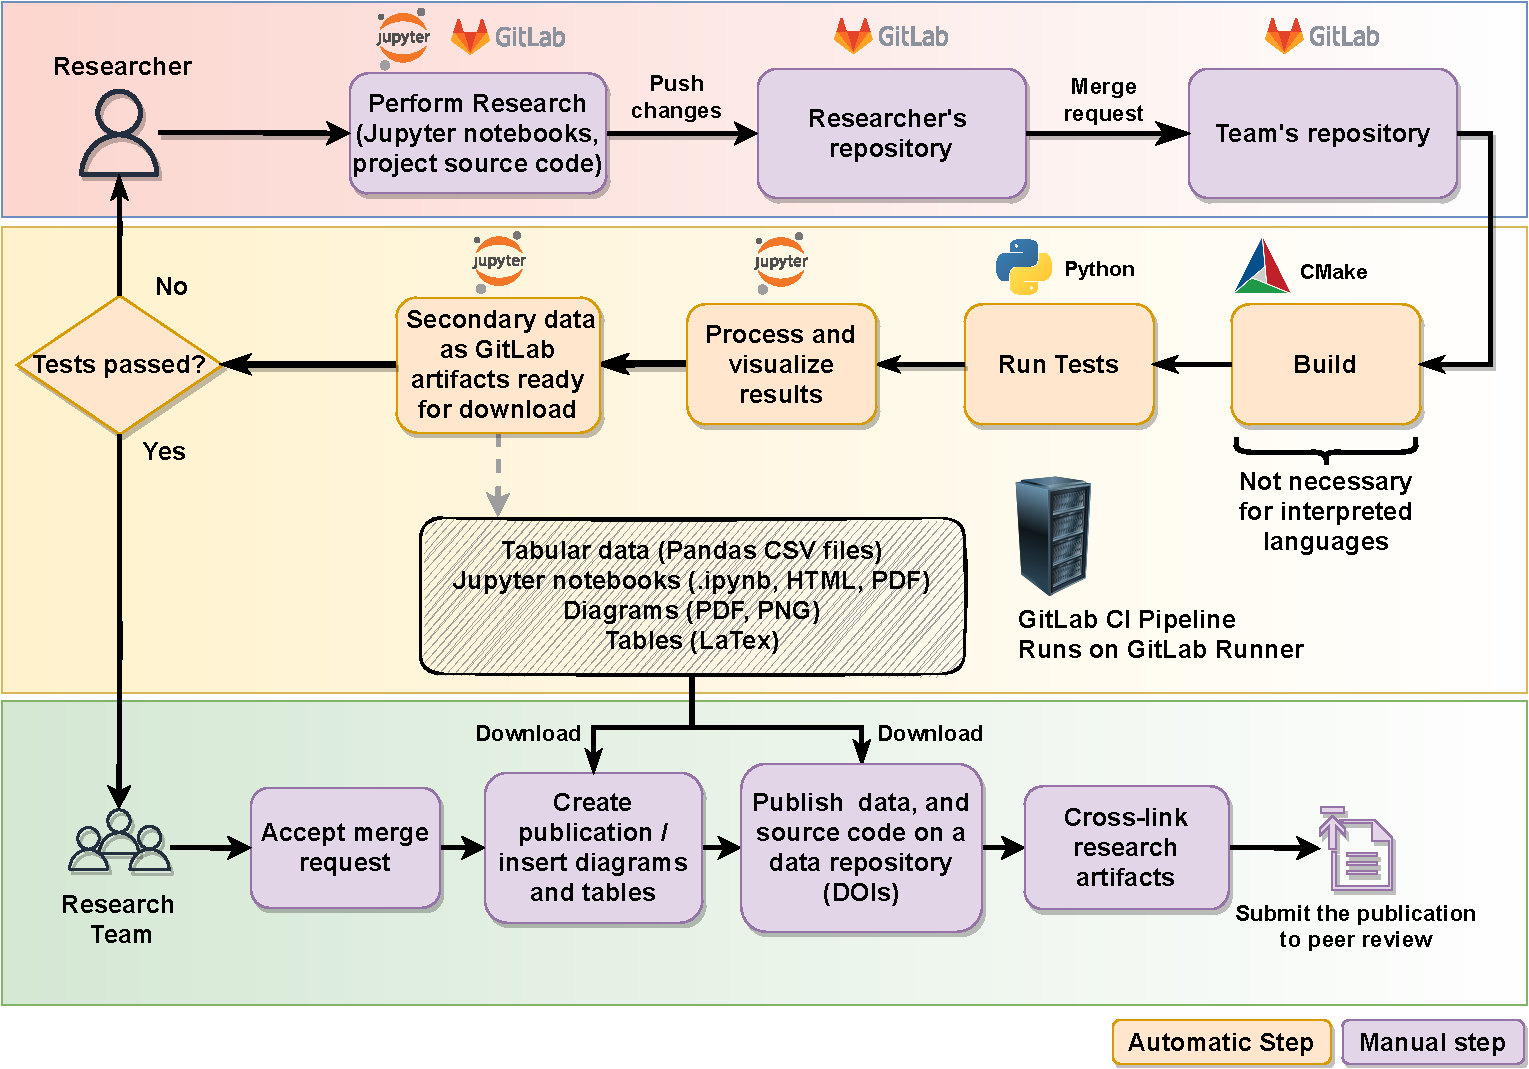
\includegraphics[width=\columnwidth]{figures/ZINF-CI-diagram.pdf}
            \end{column}
            \begin{column}[c]{0.20\textwidth}
                Working in a team.
            \end{column}
        \end{columns}
\end{frame}

\begin{frame}{(Continuous) Integration of scientific software} 
	\framesubtitle{Schematic diagram for the individual workflow}
        \vfill

        \centering

        \begin{columns}
            \begin{column}[c]{0.55\textwidth}
                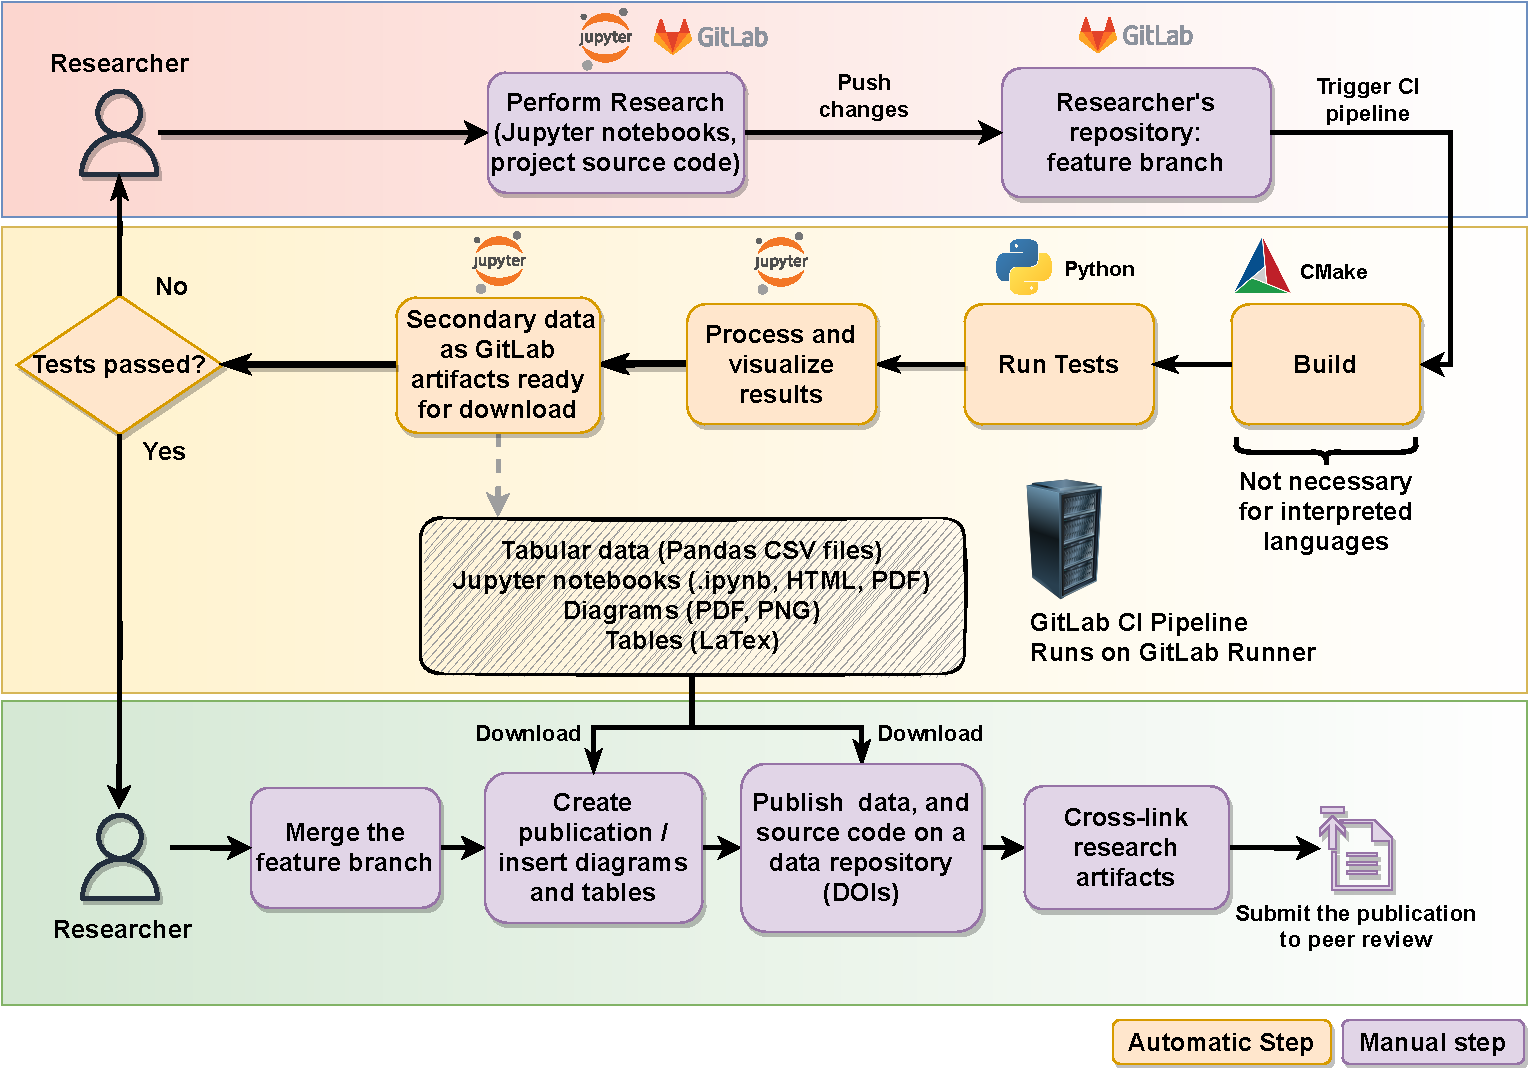
\includegraphics[width=\columnwidth]{figures/ZINF-CI-diagram-individual.pdf}
            \end{column}
            \begin{column}[c]{0.20\textwidth}
                Working alone. 
            \end{column}
        \end{columns}
\end{frame}

\begin{frame}{(Continuous) Integration of scientific software} 
\framesubtitle{CI in a nutshell I}

    \vfill

    \begin{itemize}
        \item A text (YAML) file is added to a repository, that specifies the tests (jobs) in a CI pipeline. 

        \item When the YAML file is pushed to an upstream git repository (GitLab), GitLab creates a CI pipeline from the YAML file. 
    \end{itemize}
\end{frame}

\begin{frame}[fragile]{(Continuous) Integration of scientific software} 
\framesubtitle{CI in a nutshell II}

    \begin{columns}
        \begin{column}[c]{0.5\textwidth}
            \begin{minted}[fontsize=\footnotesize]{yaml}
initialization_param_study:
  stage: running
  dependencies:
    - build_release
  script: 
    # run the parameter variation tests 
    - cd cases/initialization/3dinit
    - ./create_and_run_levelset.sh
    - ./reproduce_publication_results.sh
  artifacts:
    paths:
        - cases/initialization/3dinit/*.csv 
        - cases/initialization/3dinit/*.pdf 
            \end{minted}
        \end{column}
        \begin{column}[c]{0.5\textwidth}
            \begin{itemize}
                \item The GitLab CI uses a YAML file for the configuration of the CI pipeline. 
                \item The CI pipeline starts the right scripts in the right order: it documents the research workflow.
                \item A click of a button in a web browser reproduces results for any version of the research software.
                \item Continuous \emph{integration} is used to \emph{integrate} only those changes that improve the software and don't break existing tests.
            \end{itemize}
        \end{column}
    \end{columns}

\end{frame}

\begin{frame}[fragile]{(Continuous) Integration of scientific software} 
\framesubtitle{CI in a nutshell III}

    \vfill

    An example CI pipeline 
    \begin{figure}
        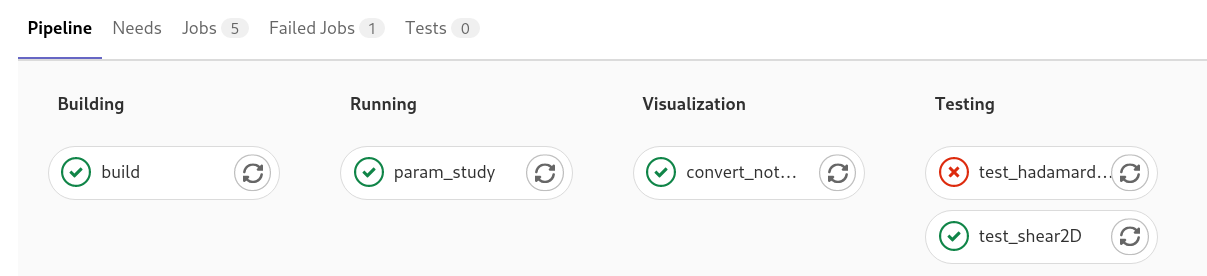
\includegraphics[width=\textwidth]{figures/pipeline-example.png}
    \end{figure}

\end{frame}

\begin{frame}{(Continuous) Integration of scientific software} 
\framesubtitle{CI in a nutshell IV}
    \vfill

    \begin{itemize}
        \item Files created within a CI job are gone when the job ends. 
        \item GitLab uses \textbf{job artifacts} to pass on data from one job to the next. 
        \item \textbf{Job artifacts can only be files stored in project's sub-folders.} 
        \item Libraries and applications are passed to other jobs as artifacts. 
        \item \textbf{Artifacts can be downloaded on the GitLab project website.}
    \end{itemize}

\end{frame}

\begin{frame}{(Continuous) Integration of scientific software} 
\framesubtitle{Running tests I}
\vfill

\begin{center}
    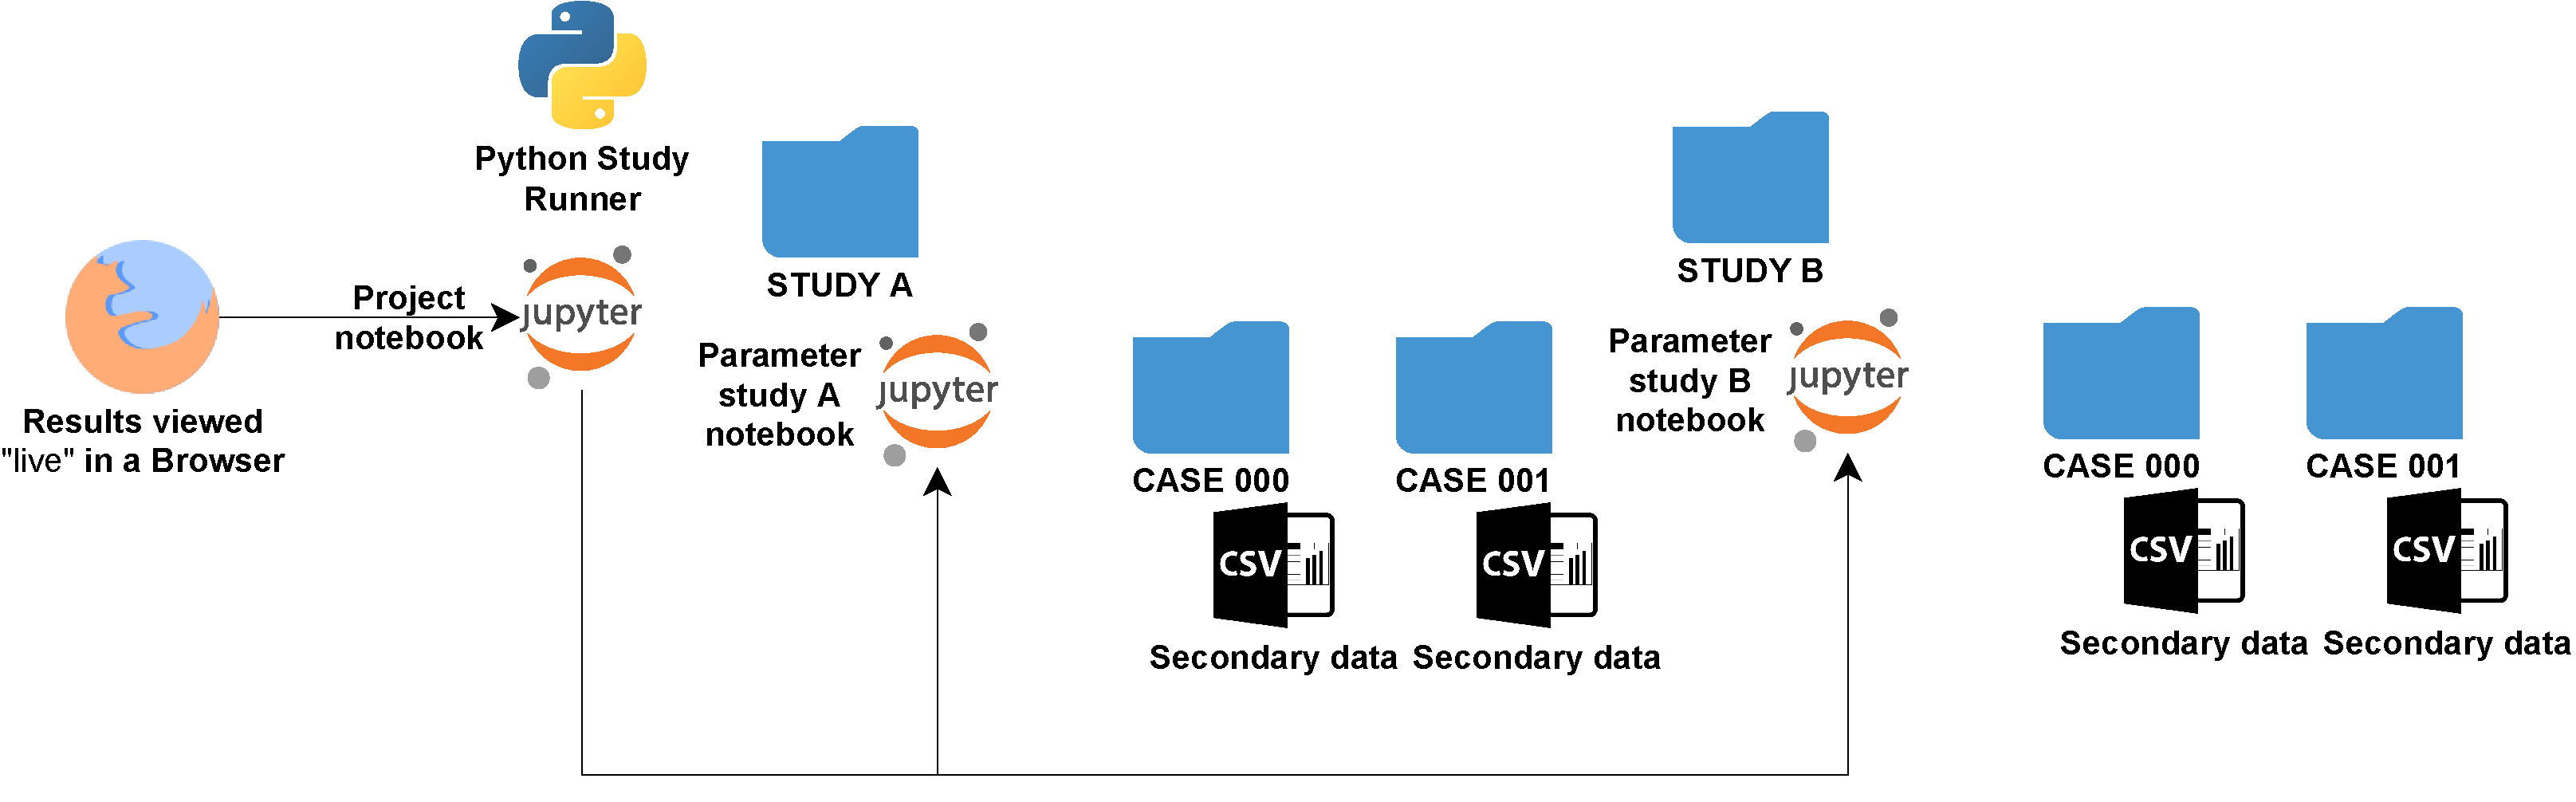
\includegraphics[width=0.9\textwidth]{figures/Cluster-Parameter-Study-Organization.pdf}
\end{center}

\end{frame}

\begin{frame}{(Continuous) Integration of scientific software} 
\framesubtitle{Running tests II}
\vfill

    \begin{itemize}
        \item Success of CSE methods is measured using verification and validation data. 
        \item Effective comparison with others (previous versions) hinges on data organization.
        \item \textbf{Goal:} being able to identify the set of study parameters used in a simulation case.
    \end{itemize}
    
    \vfill
    \begin{itemize}
        \item \textbf{Legacy code}: 
            \begin{itemize}
                \item use the existing folder structure and parameterization tools %\faGraduationCap,
                \item The mapping (case000) $\to$ (parameter vector) must be stored (YAML, ...)
            \end{itemize}
        \item \textbf{New code}: 
            \begin{enumerate}
                \item Simple folder and file structure %\faGraduationCap
                \item HDF5\footnote{\url{https://www.hdfgroup.org/solutions/hdf5}} or other open data format.
                \item Alternative to HDF5: \textbf{ExDir}\footnote{Dragly, Svenn-Arne, et al. "Experimental Directory Structure (Exdir): An alternative to HDF5 without introducing a new file format." Frontiers in neuroinformatics 12 (2018): 16.} 
            \end{enumerate}
    \end{itemize}

\end{frame}

\begin{frame}{(Continuous) Integration of scientific software} 
\framesubtitle{Running tests II}
\vfill

\begin{center}
    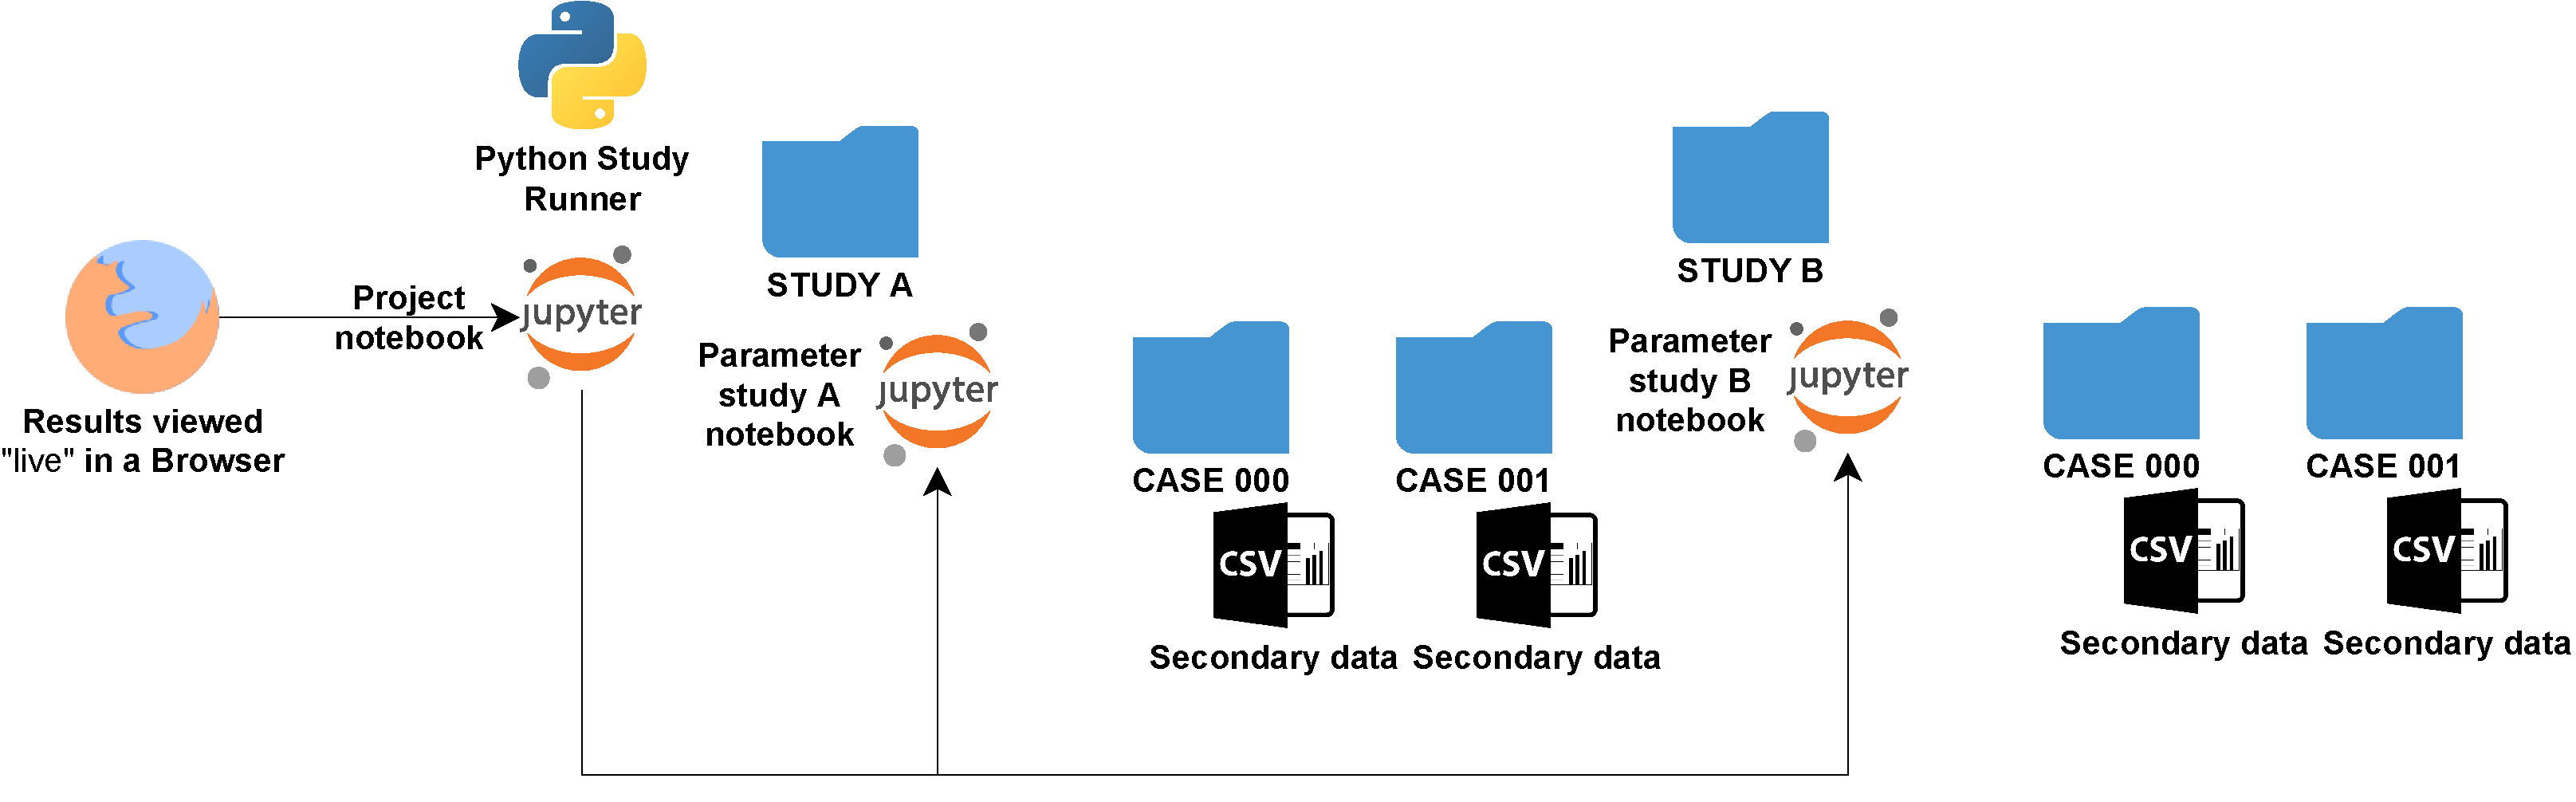
\includegraphics[width=0.9\textwidth]{figures/Cluster-Parameter-Study-Organization.pdf}
\end{center}

    \begin{itemize}
        \item Associate simulation cases with their metadata. 
        \item \texttt{\{case000 : \{N\_CELLS: 32, MODEL : shear2D\}\}}
        \item Store this information using a standard open-source format (\textbf{interoperability}).
    \end{itemize}

\end{frame}

\begin{frame}{(Continuous) Integration of scientific software} 
\framesubtitle{Running tests III}
\vfill

    Use Jupyter notebooks\footnote{\href{https://jupyter.org/}{https://jupyter.org/}} and pandas\footnote{\href{https://pandas.pydata.org/}{https://pandas.pydata.org/}} for 
    \begin{itemize}
        \item \textbf{Documentation}: geometry, initial and boundary conditions, error norms, comparison data.
        \item \textbf{Data processing}: verification errors (conservation, convergence, stability), validation errors 
        \item \textbf{Result analysis}: interactive and remote, while simulations are running!
            \begin{itemize}
                \item Jupyter notebook server can be started on a remote machine and accessed in a web browser.
            \end{itemize}
    \end{itemize}


\end{frame}

\begin{frame}{(Continuous) Integration of scientific software} 
\framesubtitle{Processing and visualizing tests}
\vfill

    \vfill

    \texttt{jupyter nbconvert notebook.ipynb --execute --to FORMAT}

    \medskip

    \begin{itemize}
        \item Agglomerate secondary data into \texttt{pandas.MultiIndex} CSV files. 
        \item Run each jupyter notebook in the repository.
        \item Export secondary data and notebooks in different formats as artifacts.
        \item \textbf{Visualization} 
            \begin{itemize}
                \item Download the artifact and open the notebook \faGraduationCap.
                \item Notebooks contain information on failing tests. 
                \item Mapping "caseID" $\to$ "parameters" is crucial for re-starting failed parameter variations! 
            \end{itemize}
    \end{itemize}

\end{frame}

\begin{frame}{(Continuous) Integration of scientific software} 
\framesubtitle{Secondary data I}
\vfill

    \begin{itemize}
        \item Data used for diagrams and tables in a publication.
        \item Data we compare our results with.
        \item Primary data: complete simulation results / experimental measurements.
    \end{itemize}

\end{frame}

\begin{frame}{(Continuous) Integration of scientific software} 
\framesubtitle{Secondary data II}
\vfill

    \href{https://pandas.pydata.org/}{pandas.MultiIndex} CSV with metadata for secondary data
    \begin{itemize}
        \item \texttt{pandas.MultiIndex} saved in "metadata columns". 
        \item \textcolor{red}{\textbf{Metadata is repeated}}: not an issue for the small secondary data! 
        \item Metadata in columns $\to$ \texttt{pandas.MultiIndex} $\to$ strongly simplified data analysis. 
        \item \textbf{Direct readable export of tables to LaTex!}
    \end{itemize}

    \footnotesize

    \begin{tabular}{llllll}
        \toprule
        {} &         H &     L\_INF &  O(L\_INF) &  EPSILON\_R\_EXACT\_MAX &  O(EPSILON\_R\_EXACT\_MAX)  \\ 
        VELOCITY\_MODEL &           &           &           &                      &                        \\ 
        \midrule
        \textcolor{red}{\textbf{SHEAR\_2D}}       &  0.125000 &  0.032961 &  1.833407 &             0.032961 &                1.833407 \\ 
        \textcolor{red}{\textbf{SHEAR\_2D}}       &  0.062500 &  0.009249 &  1.955529 &             0.009249 &                1.955529 \\ 
        \textcolor{red}{\textbf{SHEAR\_2D}}       &  0.031250 &  0.002385 &  1.988745 &             0.002385 &                1.988745 \\ 
        \textcolor{red}{\textbf{SHEAR\_2D}}       &  0.015625 &  0.000601 &  1.997178 &             0.000601 &                1.997178 \\ 
        \textcolor{red}{\textbf{SHEAR\_2D}}       &  0.007813 &  0.000150 &  1.999294 &             0.000150 &                1.999294 \\ 
        \textcolor{red}{\textbf{SHEAR\_2D}}       &  0.003906 &  0.000038 &  1.999294 &             0.000038 &                1.999294 \\ 
        \bottomrule
    \end{tabular}

\end{frame}

\begin{frame}{(Continuous) Integration of scientific software} 
\framesubtitle{Cross-linking I}
\vfill

    \begin{center}
            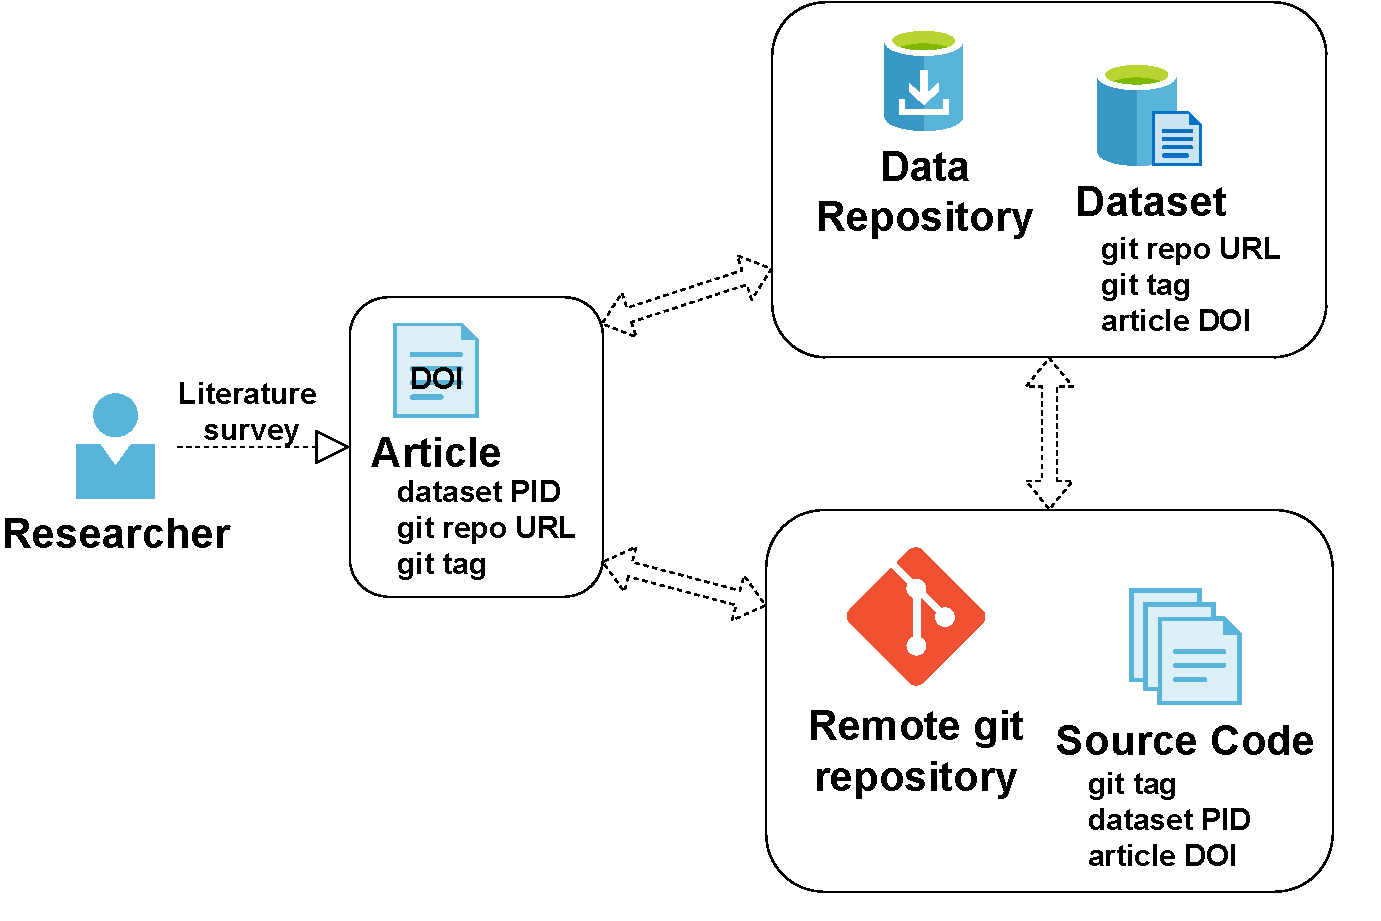
\includegraphics[width=0.67\textwidth]{figures/cross-linking.pdf}
    \end{center}

\end{frame}

\begin{frame}{(Continuous) Integration of scientific software} 
	\framesubtitle{Schematic diagram for the individual workflow}
        \vfill

        \centering

        \begin{columns}
            \begin{column}[c]{0.55\textwidth}
                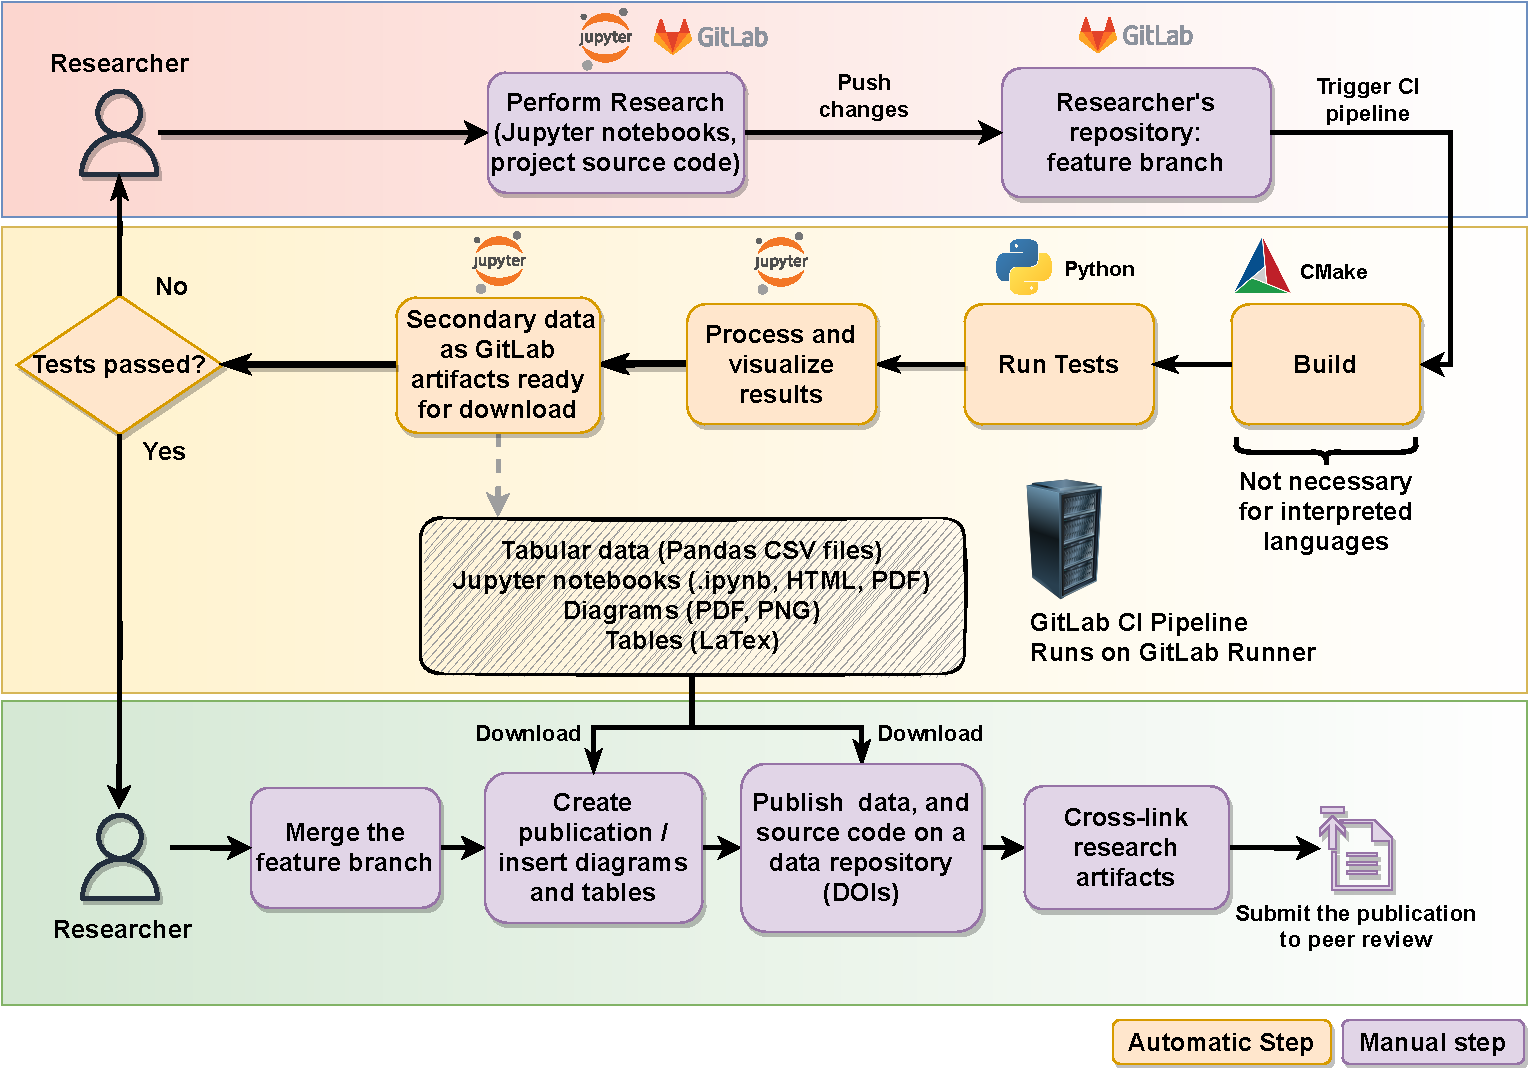
\includegraphics[width=\columnwidth]{figures/ZINF-CI-diagram-individual.pdf}
            \end{column}
            \begin{column}[c]{0.20\textwidth}
                Working alone. 
            \end{column}
        \end{columns}
\end{frame}

\begin{frame}{(Continuous) Integration of scientific software} 
\framesubtitle{Cross-linking II}
\vfill

    Cross-linking is done manually. 
    \begin{itemize}
        \item Place whatever you can under version control. 
        \item \textbf{When a set of milestones is reached (\emph{release})} , use \href{https://git-scm.com/book/en/v2/Git-Basics-Tagging}{git-tags} as version snapshots, and upload the research data to a data repository, e.g. \href{https://tudatalib.ulb.tu-darmstadt.de/}{TUDatalib} at TU Darmstadt, or \href{https://zenodo.org/}{Zenodo}.
            \begin{itemize}
                \item Secondary data (diagrams, tables), raw data (simulations, experiments), archive of the research software, ...
            \end{itemize}
        \item Data uploaded to a data repository is associated with Persistent Identifiers (PIDs), e.g. DOIs.
        \item Cite the research data using DOIs in the report (article, preprint).
        \item Upload the report to a pre-print repository, e.g. \href{https://arxiv.org/}{ArXiv}. 
        \item Edit the data on the data repository and mention the arXivID.  
        \item Submit the pre-print to a journal for peer-review.
    \end{itemize}

\end{frame}


\begin{frame}[fragile]{Continuous Integration of Scientific Software}
    \framesubtitle{Cross-linking III} 
    \vfill

    \begin{itemize}
        \item \textbf{Research software has been improved} if the results have been improved \textbf{with respect to a previous or competing publication.}
        \item A major milestone are improved results for a set of verification / validation tests.
        \item The cross-linking therefore revolves around the publication (pre-print, report, ...). 
        \item The cross-linking makes it possible to find the version of research software used to generate the results in the publication: repository link + git tag, repository snapshot, software image. 
        \item Once the version is found, CI automatically reproduces all results from the publication with a click of a button.
    \end{itemize}

\end{frame}

\begin{frame}{(Continuous Integration with result visualization)} 
    \framesubtitle{Test evaluation}

    \vfill

    Very straightforward 
    \begin{itemize}
        \item Python scripts test secondary data agglomerated by notebooks from simulation results.
        \item \textbf{Examples:} 
            \begin{itemize}
                \item Is the order of convergence of an error norm $\ge 2.0$?
                \item Is is the difference between simulation and experiment data $\le 4\%$? 
            \end{itemize}
    \end{itemize}

\end{frame}


\begin{frame}{(Continuous) Integration of scientific software} 
    \framesubtitle{Docker (containerization)}
    \vfill

    \begin{columns}
        \begin{column}[c]{0.4\textwidth}
            \begin{center}
            \only<1>{
                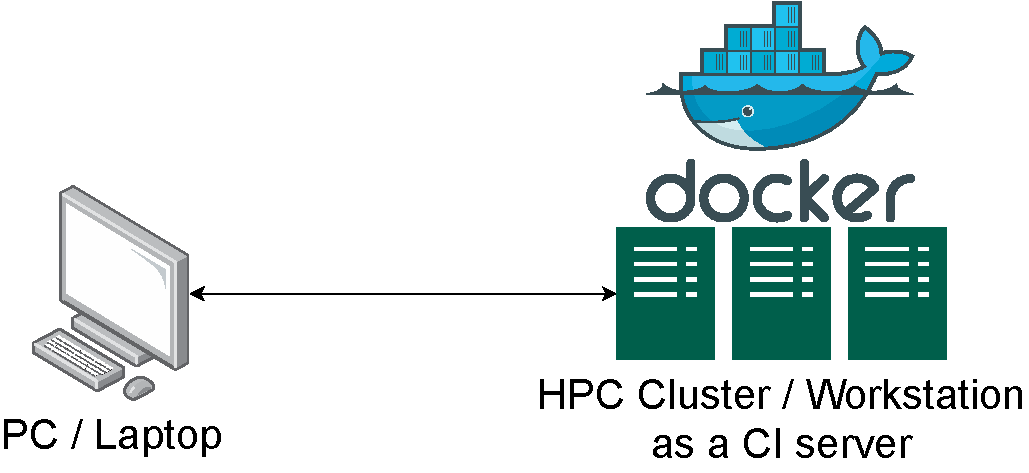
\includegraphics[width=\columnwidth]{figures/ci-with-docker.pdf}
            }
            \only<2>{
                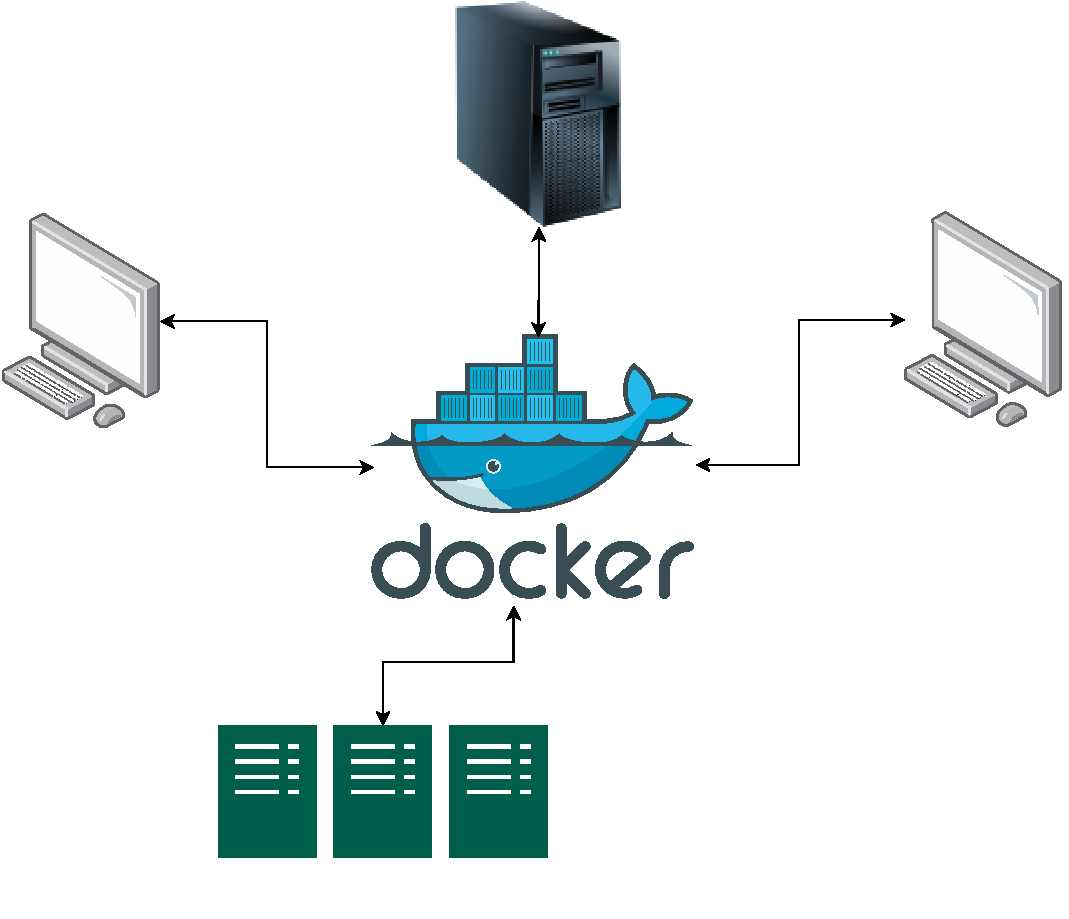
\includegraphics[width=\columnwidth]{figures/docker-description.pdf}
            }
            \end{center}
        \end{column}
        \begin{column}[c]{0.6\textwidth}
            \begin{itemize}
                \item Instead of installing the research software only on the laptop/PC and the HPC cluster / workstation, we install it in a virtual environment - \textbf{a Docker image}.
                \item The Docker image then works on any machine that runs Docker. 
                \item Sharing research software becomes trivial - if our colleague wants to use our software, no installation (besides Docker) is required. 
            \end{itemize}
        \end{column}
    \end{columns}

\end{frame}

\begin{frame}{(Continuous) Integration of scientific software} 
\framesubtitle{Computing resources}
\vfill

    \vfill
    The GitLab CI requires a \textbf{runner}: a machine that runs the CI jobs.
    \begin{enumerate}
        \item \textbf{Short few CPU-core tests}: work-PC \faGraduationCap.    
        \item \textbf{Short many-core tests}: obtain a workstation with a 64-Core CPU\footnote{Thanks to \href{https://www.sfb1194.tu-darmstadt.de/index.en.jsp}{CRC 1194 at TU Darmstadt.}}\faGraduationCap.
        \item \textbf{HPC tests}: combine 1. or 2. with an HPC cluster. 
    \end{enumerate}

    An HPC cluster is relevant for production tests and performance measurements.
    \begin{itemize}
        \item This workflow uses coarse ("smoke") tests \faGraduationCap
            \begin{itemize}
                \item Unit tests run for 1. and 2.
                \item Convergence ensured for 1. and 2.
                \item Is efficient in parallel for 1. and 2. 
            \end{itemize}
        \item \textbf{Challenge}: Is it possible to combine 1., 2. and 3. and publish instead of perish \faGraduationCap?
    \end{itemize}

\end{frame}

\begin{frame}{(Continuous) Integration of scientific software} 
    \framesubtitle{A GitLab runner with a Docker executor and a local Docker image}

    \vfill 
    Build a Docker image for your software, and track the Dockerfile with the project.\\
    \medskip
    \href{https://gitlab.com/tmaric/fvc-reconstruct/-/tree/main/docker}{Example OpenFOAM Dockerfile} on \texttt{ubuntu:focal} with "system" open-mpi and scotch.

    \medskip
    On the testing machine
    \begin{itemize}
        \item Install Docker and GitLab runner and register the GitLab runner with a Docker executor.
        \item Configure the GitLab runner in \texttt{/etc/gitlab-runner/config.toml} to
            \begin{itemize}
                \item use a local Docker image, e.g., \texttt{image = "openfoam-v2012\_ubuntu-focal:latest"}, and
                \item never pull images \texttt{pull\_policy = never}.
            \end{itemize}
    \end{itemize}

\end{frame}

\begin{frame}{(Continuous) Integration of scientific software} 
    \framesubtitle{Summary I}

\begin{columns}
    \begin{column}[c]{0.51\textwidth}
        \centering
        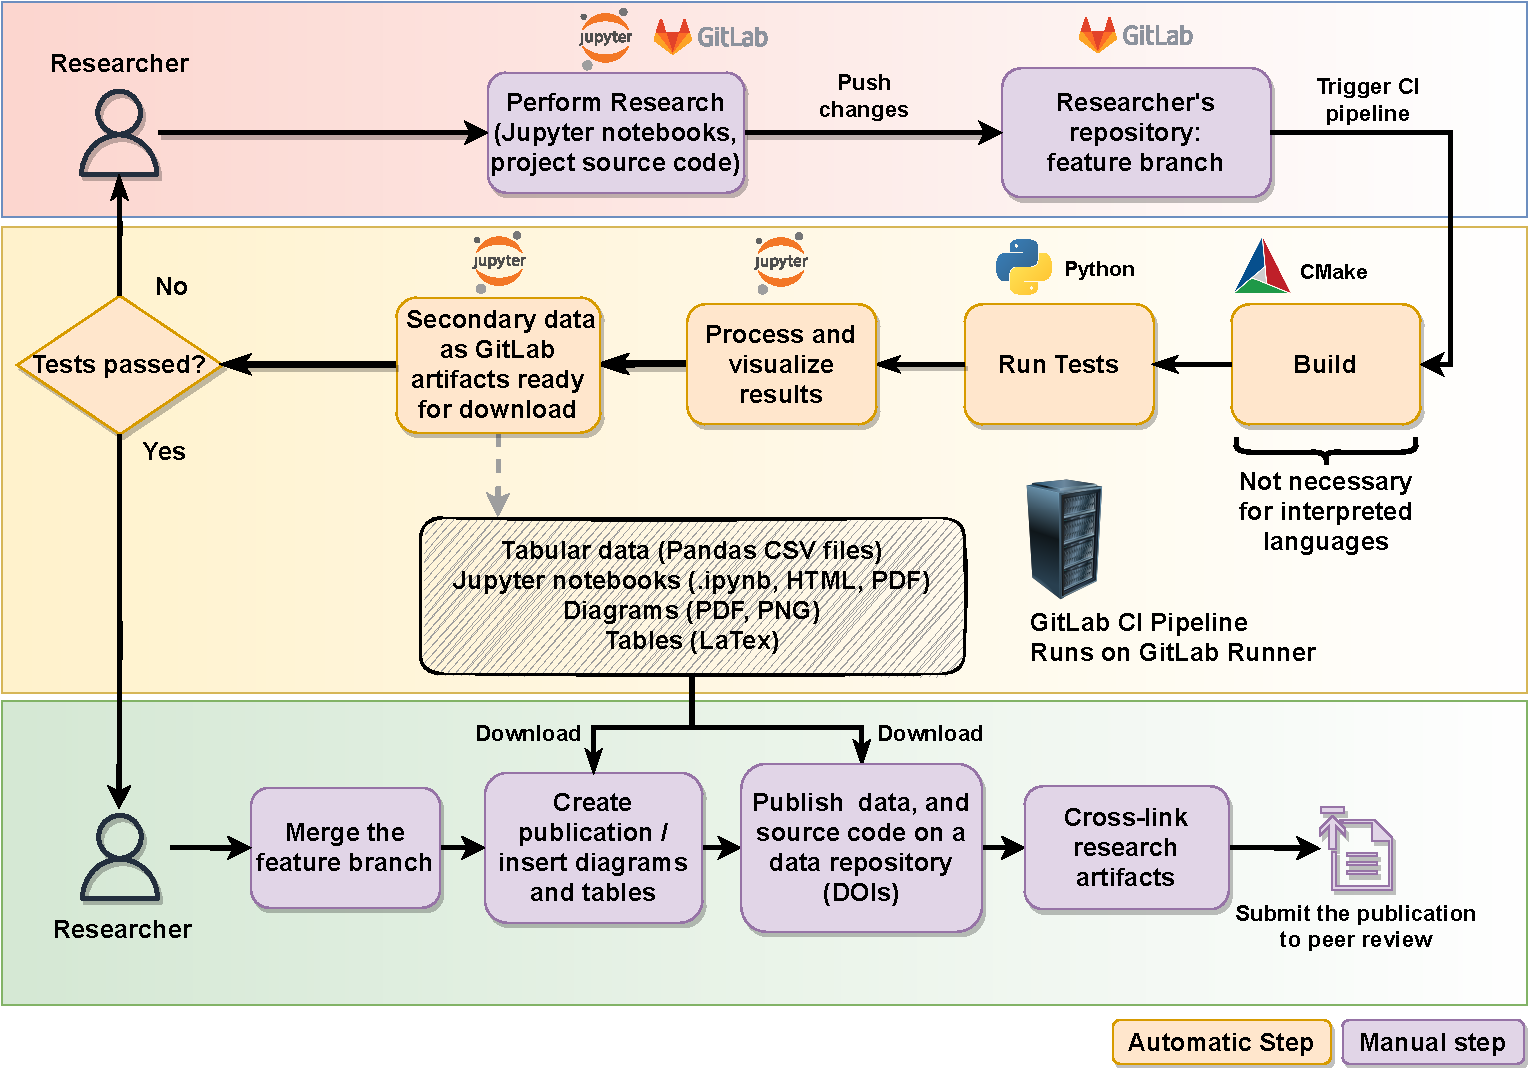
\includegraphics[width=\columnwidth]{figures/ZINF-CI-diagram-individual.pdf}
    \end{column}
    \begin{column}[c]{0.49\textwidth}
        \footnotesize
        \begin{algorithmic}[1]
            \State Track changes using version-control.
            \While{Milestone not reached}
                \For{study in studies} \Comment On an HPC cluster.
                    \State Automate data processing and visualization.
                    \State Run study.
                    \State Check results and apply code changes. 
                \EndFor
                \If{results are improved on the HPC cluster} 
                    \State Push changes to the remote repository. 
                    \If{CI pipeline tests pass}
                        \State Milestone reached.
                        \State Add new tests to the CI pipeline, 
                        \State Merge feature into development branch. 
                        \State Cross-link publication, data, and source code.
                    \EndIf
                \EndIf
            \EndWhile
        \end{algorithmic}
    \end{column}
\end{columns}

\end{frame}

\begin{frame}{(Continuous) Integration of scientific software} 
    \framesubtitle{Summary II}

\end{frame}

\begin{frame}{(Continuous) Integration of scientific software} 
\framesubtitle{Similarity with other workflows / best practices}

	\vfill
	Our \emph{(subjective)} estimates* of similarity $1-5$ (higher is more similar), $-$: aspect not addressed.
	\begin{center}
		\scriptsize
		\begin{tabular}{@{} *6l @{}}    \toprule
				\emph{DOI} & \emph{Branching model} & \emph{TDD} & \emph{Cross-linking} & \emph{CI}  & (Meta)data standardization \\\midrule
				 \href{https://doi.org/10.12688/f1000research.11407.1}{10.12688/f1000research.11407.1} 
					 & -  & -  & -  & - & 1  \\ 
				 \href{https://doi.org/10.3934/math.2016.3.261}{10.3934/math.2016.3.261} 
					 & -  & -  & -  & - & 2  \\ 
				 \href{https://doi.org/10.1371/journal.pbio.1001745}{10.1371/journal.pbio.1001745} 
					 & 1  & 2  & -  & - & -  \\ 
				 \href{https://doi.org/10.1371/journal.pcbi.1005510}{10.1371/journal.pcbi.1005510}
					 & -  & -  & 3 & 1 & 3  \\ 
				 \href{https://doi.org/10.1145/2723872.2723881}{10.1145/2723872.2723881}
					 & 1  & -  & - & 1 & -  \\ 
				 \href{https://dl.acm.org/doi/10.1145/3324989.3325719}{10.1145/3324989.3325719}
					 & 1  & -  & - & 5 & -  \\ 
				 \href{https://doi.org/10.1371/journal.pone.0230557}{10.1371/journal.pone.0230557}
					 & 1  & -  & - & 1 & 4  \\ 
				 \href{https://doi.org/10.1145/3219104.3219147}{10.1145/3219104.3219147} 
					 & 1  & -  & -  & 4 & - \\\bottomrule
				 \hline
		\end{tabular}
	\end{center}
	
	*\emph{The list may still be incomplete.}
	
\end{frame}

%\begin{frame}[fragile]{(Continuous Integration with result visualization)} 
    %\framesubtitle{Building OpenFOAM projects or projects with out-of-source installation}

    %\vfill
    %\textbf{Out-of-source installation}: binaries only available outside the repo! 
    %\begin{itemize}
        %\item \textbf{Use environment variables to build and pass on artifacts} 
        %\item \texttt{\$FOAM\_USER\_LIBBIN} folder stores library binaries. 
        %\item \texttt{\$FOAM\_USER\_APPBIN} folder stores application binaries. 
        %\item \textbf{Build job}: 
            %\begin{itemize}
                %\item create artifact folders inside the repo, 
                %\item copy library and application binaries to artifact folders, 
                %\item export artifact folders. 
            %\end{itemize}
        %\item \textbf{Run job: \textbf{simplified} copying of binary artifacts to OpenFOAM folders}
            %\begin{itemize} 
                %\item \texttt{mkdir -p} \texttt{\{\$FOAM\_USER\_LIBBIN, \$FOAM\_USER\_APPBIN\}}
                %\item \texttt{cp FOAM\_USER\_LIBBIN/* \$FOAM\_USER\_LIBBIN} 
                %\item \texttt{cp FOAM\_USER\_APPBIN/* \$FOAM\_USER\_APPBIN} 
                %\item Run tests.
            %\end{itemize}
    %\end{itemize}


%\end{frame}


%\begin{frame}{(Continuous Integration with result visualization)} 
    %\framesubtitle{Example}

    %\vfill
    %\begin{center}
        %\href{https://gitlab.com/tmaric/fvc-reconstruct/-/pipelines/279564790}{Example OpenFOAM CI project} 
    %\end{center}

%\end{frame}
